
%%% INITIAL SUMMARY

The study of neurodegenerative diseases such as Alzheimer's disease (AD) usually entails gathering different markers of the disease coming from different sources or metodologies \cite{Jack2010}: brain imaging techniques, cognitive assessments, or cerebrospinal fluid punctures. Over the past decades, such techniques have become widespread and there has been a surge on the number of available data. Large datasets from patients at different stages of the disease containing heterogeneous and over time (longitudinal) data could help unravel unseen mechanisms and provide insights on its evolution. However, we need novel methods that can leverage and extract meaningful information from such complex data. \\

Machine learning (ML) is a set of techniques and models that have shown strong performance on a variety of tasks. These techniques are closely related to statistical methods and have gained a lot of popularity recently with the advent of deep learning (DL) \cite{LeCun2015}. ML and DL techniques have been applied to medical data, including AD \cite{Litjens2017,Ching2018}. The field still faces many challenges, and it will keep developing over the next years. An important challenge is to build methods that are able to find relationships between different markers to improve our understanding of the progression of the disease. In this thesis, we explore machine learning and statistical methods that are able to help us gain insight on different aspects of AD using heterogeneous, longitudinal medical data. \\

\section{Alzheimer's disease}

% Severity of Alzheimer's Disease.
AD is an incurable neurodegenerative disease that causes a progressive degeneration of the brain and cognitive functions \cite{Lane2018}. Our current understanding is that the disease is characterized by an accumulation of amyloid-beta (A$\beta$) proteins in the brain and the formation of tau plaques, that causes brain atrophy and gradually impair the cognition of the patients, and finally leading to death \cite{Ballard2011}. AD affects more than 47 million people worldwide, generating an estimated healthcare cost of around 604 billion US dollars a year \cite{AlzheimersAssociation}. As AD is a disease that generally affects elderly people, and accounting for the general aging of the population, this impact will only get stronger. It is estimated that, by 2030, 76 million people worldwide could be affected by this disease \cite{AlzheimersAssociation}. \\

%% Small paragraph on the difference between familial AD and late onset AD.
Generally, when we talk about AD we refer to sporadic late-onset AD, which has no known cause. There also exists a variant named autosomal dominant familial AD, affecting less than $5\%$ of AD patients \cite{Bird1993}, which is caused by genetic mutations on APP, PSEN1 and PSEN2 genes \cite{Campion1999}. It has an earlier age of onset, but it has a similar clinical presentation compared to its sporadic, most common form \cite{Ryan2016}. All the work contained in this thesis is only applied to late-onset AD, and from now on it will be referenced in the text as AD for simplicity. \\

%% use marinescus thesis citations
Up to now, there has been no successful treatment to cure or slow down the cognitive decline caused by AD. Despite all the research on the topic, all clinical trials have failed \cite{Mehta2017} and did not manage to prove efficacy, even recent ones \cite{Huang2020}. Failures in drug design and development for AD could be linked to many reasons. One is that our understanding of the underlying processes that initially cause the cascade of events leading to the disease still needs to improve. Another reason could be that any potential successful drug would need to be administered at a presymptomatic stage of AD \cite{Mehta2017,Huang2020}. Detection of cognitively healthy patients at risk, or patients with very mild impairment that will progress to AD in the future is of utmost importance for future drugs and trials. \\ 

In the literature, diagnosis of patients is usually divided in three stages \cite{Brookmeyer2007}, although other classifications have been recently proposed \cite{Jack2018}:

\begin{enumerate}\itemsep5pt
\item Healthy control or cognitively normal (CN), when the patient shows neither signs of the disease nor cognitive problems.
\item Mild cognitive impairment (MCI), when the patient shows signs of cognitive impairment. It can be divided into two substages: early MCI and late MCI, differentiating between patients by their degree of cognitive impairment.
\item AD, when the patient is considered to have completely progressed into full-blown dementia.
\end{enumerate}

\subsection{AD markers}

To determine the current stage of the disease, various markers describing key pathophysiological processess of AD have been proposed over the years. AD is a multifactorial disease, with distinct progression paths depending on the used markers. AD is characterized by protein amyloid-beta (A$\beta$) deposition in the brain \cite{Rissman2012}, tau injury, and structural neurodegeneration \cite{Jack2013}. Those three indicators precede cognitive impairment, leading to death. For the measurement of these indicators, different markers have been proposed:

\begin{enumerate}\itemsep5pt
\item Brain A$\beta$ deposition in the brain can be detected both in positron emission tomography (PET) imaging \cite{Clark2011}, and in cerebrospinal fluid (CSF) \cite{Andreasen1999}.
\item Tau injury and dysfunction caused by tau and p-tau plaques, found in tau-PET imaging and CSF \cite{Andreasen1999,Blennow2010}.
\item Neurodegeneration provoked by tau injury. It can be observed in structural magnetic resonance imaging (MRI) \cite{Weiner2005} and in fludeoxyglucose (FDG)-PET imaging \cite{Chetelat2003}.
\item Memory and cognition, measured by cognitive tests.
\end{enumerate}

%% Screening
The main screening tool for clinical assessment of AD is the clinical interview between the patient and the doctor, where the severity of the cognitive problems of the patient can be assessed, followed by a cognitive physical examination to capture the aforementioned markers and assess the presence of the disease \cite{Lane2018}. \\

%% Blood based
Apart from the aforementioned markers and imaging techniques, blood based markers have also been proposed for AD diagnosis \cite{Shi2018}, as they potentially could be a non-invasive, cheaper way to diagnose. Recently, plasma marker p-tau181 has shown promising results for an accurate AD diagnosis \cite{Karikari2020}. \\

%% APOE
AD has also been linked to several genetic mutation risks. Apart from the genes linked to previously mentioned autosomal familial AD, the major genetic risk factor for AD is the Apolipoprotein E (APOE) $\varepsilon$4 allele \cite{Saunders1993}. It has been linked to an increased risk of AD, depending on allele load (if the patient has one or two copies of the allele) \cite{Liu2013a}.

\subsection{Longitudinal marker dynamics and disease model}

The previous markers can be studied and modelled longitudinally. Modelling their trajectories and progression can give us more insight on how they change and interact. For example, longitudinal data analysis on MRI allows us to calculate the rate of change of specific brain structures, such as the dynamics of cortical and hippocampal atrophy. \\

A widely accepted progression model of AD was proposed by \cite{Jack2010}. Their model is based on marker evolution, where each marker progresses from normal values to abnormal values differently. The order of the markers is the presented above: A$\beta$ deposition, followed by tau injury, neurodegeneration and cognition. Empirical data and experiments reviewed in \cite{Jack2013} confirm the validity of the model, although other data-driven works do not fully agree with it \cite{Iturria-Medina2016}. \\

%% Explicar aqui una mica de AD subtyping, del paper de young, tal tal
AD is a highly heterogeneous disease. It can overlap with other neurological pathologies and presenting different paths of neurodegeneration, with different rates of atrophy for different areas of the brain \cite{Lam2013,Poulakis2018}, distinct clinical and cognitive characteristics \cite{Murray2011} or even differences in other more specific markers like CSF proteomics \cite{Tijms2020}. Development of methods to study the progression of AD should also take into account this heterogeneity for a better understanding of the disease. \\

\section{Challenges in longitudinal and heterogeneous data}

Longitudinal data are composed of sequential data acquisitions for subjects over a period of time. This contrasts with cross-sectional studies, which focus on single acquisitions per subject. Here, we describe the main characteristics and analysis challenges that arise while dealing with longitudinal data. \\

Two sources of variability can be defined for a longitudinal study in a cohort of subjects: the inter-subject variability, i.e., the differences between observations of different subjects, and the intra-subject variability, i.e., the differences between observations of a same subject, which tend to be highly correlated compared to the former. Those two sources of variation give valuable information about the progression of the disease between- and within- subjects. In cross-sectional studies, those two variabilities are non-separable: given two samples of different subjects, it is not possible to know to what extent their variation is due to inter-subject variability or to the different stages of the disease. Adding longitudinal samples for each subject allows us to distinguish between those two variabilities, improving our understanding of the disease \cite{Fitzmaurice2008}. \\

\begin{figure}[htbp]
  \centering
  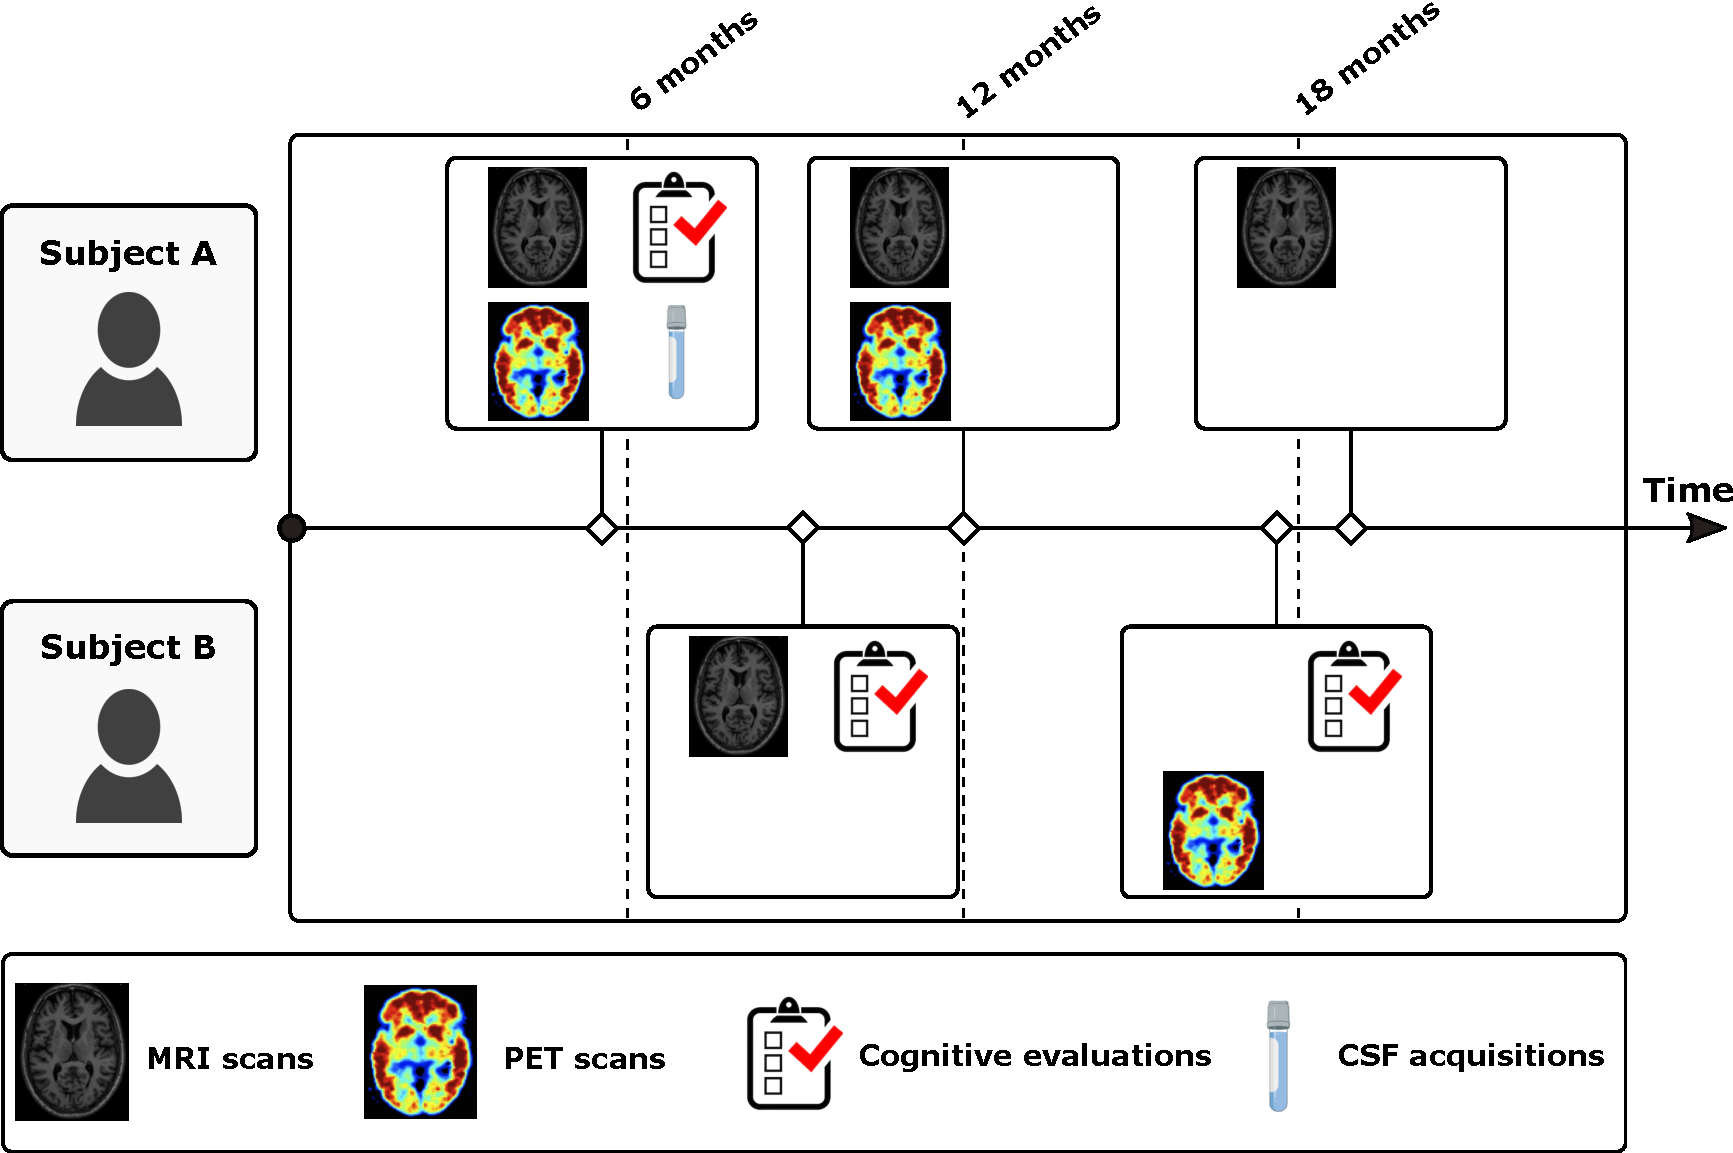
\includegraphics[width=1.0\textwidth]{figures/introduction/Fig-progression.pdf}
  \caption{Longitudinal representation of data acquisitions for two patients.}
  \label{long}
\end{figure}

Figure \ref{long} shows an example of a longitudinal study for two subjects, with multiple data modalities, over a fixed span of time. It illustrates some of the challenges that can appear in a longitudinal, multimodal data study: \\

% The figure should include these various points
% \itemsep5pt was put originally but tal
\begin{enumerate}
\item Each subject can have a different number of acquisitions, leading to an unbalanced data problem. In the figure, Patient B missed the 12th month acquisition for some reasons.
\item There can be missing data due to missing acquisitions from some modalities. In the figure, only patient A at the 6-months follow-up has all the acquisitions.
\item Data are not necessarily acquired at the same time point for the different subjects.
\item Time spacing between follow-ups can be variable, even within a single subject.
\end{enumerate}

Another problem, not shown in the figure, is that different patients can be at different stages of the disease at a given time point. Reference time to measure progression remains an open issue in the field \cite{Ashford2001}.  \\

Protocols of data acquisition try to palliate these problems, but in a clinical setting, this is very difficult to achieve: sometimes patients miss their scheduled screening session and data cannot be gathered. Other patients might drop out from the study for a variety of reasons, such as disease severity or moving out of the city/country, and in other cases, data of a given time point could need to be discarded because of quality problems. For these reasons, most of the available longitudinal data is unbalanced. \\

\subsection{Studies and initiatives} 
%% Explain about studies that focus on longitudinal data. and about the challenges that promote the use of longitudinal data for progression of the disease.

There has been a remarkable number of initiatives to promote using longitudinal data on AD modelling. Availability of patients' longitudinal data is key to study the progression of the disease. Lawrence et al. \cite{Lawrence2017} presented a review of available longitudinal AD biomarker datasets, finding that more efforts are needed to increase the follow-up duration, increase the population sizes and standardize the acquisition methods. One of the largest studies is the Alzheimer's Disease Neuroimaging Initiative (ADNI) \cite{Mueller2005}, a multimodal, ongoing longitudinal study with hundreds of enrolled subjects, gathering imaging data, cognitive scores, blood and CSF markers. To unify and share the available data, the Alzheimer's Association has created The Global Alzheimer’s Association Interactive Network (GAAIN)\footnote{\url{http://www.gaain.org}} to share data between independent studies and build collaborations to create and explore large, heterogeneous cohorts. More recently, a new initiative named Alzheimer's Disease Data Initiative (ADD)\footnote{\url{https://www.alzheimersdata.org/}} have been created for similar reasons of data unification and sharing. \\

\section{Machine learning for medical data}

%% Introductory paragraph: general citations on healthcare: medical records, image segmentation, top results from google, etc.
Traditional methods for data analysis usually rely on searching relationships between measured quantities (e.g. variables). For example, in statistical inference, we start from a hypothesis of the effect of an independent variable on the dependent (output) variables, and look for relevant associations that confirm or refute the hypothesis. From another perspective, ML allows us to accurately model the relationship between input and output that generalize to unseen data. ML is particularly helpful when dealing with complex and unwieldy data, and when the number of input variables is large. Usually, ML models are trained for a specific task (e.g. image recognition, or diagnosis prediction), but such techniques are also very useful to find patterns or relationships in high-dimensional data that could not be found otherwise due to the inherently complex nature of it. Lately, DL has become one of the most used ML tools for high-dimensional data. \\

ML has been applied to many healthcare problems. For example, breast cancer screening \cite{McKinney2020} or predicting cardiovascular risk factor on retina images \cite{Poplin2018}, have shown strong results using ML based techniques. A very prolific application of ML is medical imaging, where it has been used for image classification, segmentation, or synthetic data generation \cite{Litjens2017}. Use of such techniques also raise important technical and ethical questions, such as privacy concerns over data usage \cite{Yang2019} or bias or transparency issues \cite{Karikari2020, Haibe-Kains2020}. Nonetheless, the results achieved show their strength and potential for problems with high-dimensional, complex medical data. \\

ML has also been used in AD research for several tasks, such as diagnosis classification \cite{Rathore2017}, disease progression modeling \cite{Oxtoby2017} or disease subtpying \cite{Young2017}, to name a few. The inherent complexity between the different modalities of markers of the disease and their temporal evolution and trajectories, coupled with the still unknown mechanisms underlying AD, make ML a prime candidate for the study of the disease. \\

%% Here, talk on the limitations of the current methods

\section{Contributions and outline of the thesis}

The main contributions of the thesis are presented in four main chapters, in addition to the introduction (Chapter \ref{ch:1-introduction}) and a final chapter with the general conclusions of our work (Chapter \ref{ch:6-conclusions}):

\begin{itemize}
    \item Chapter \ref{ch:2-review} reviews statistical and machine learning applications in AD using longitudinal neuroimaging. We perform a literature review of the field, selecting 105 papers to review. Our objective was to paint a clear picture of the state of the field, compare the current approaches and methods, and discover existing limitations. We show that methods that use longitudinal data have a strong potential for modelling disease progression and computer-aided diagnosis. 
    \item Chapter \ref{ch:3-cimlr} shows a study on AD subtyping using blood markers. We apply a non-supervised clustering approach, based on multiple kernel learning, to study AD subtyping using novel plasma markers. We obtain different subtypes of patients with different presentation of the disease, and we discover potential interactions between the groups using MRI based markers.
    \item Chapter \ref{ch:4-rnnvae} presents a generative model based on variational autoencoders and recurrent neural networks that is able to combine multimodal, longitudinal data, with variable number of time-points.This method can predict the evolution of a given patient, show relationships between modalities, and input missing channels. This is achieved by explicitly modelling the interdependencies between modalities, and using recurrent neural networks to model the evolution of each modality over time. We show the potential of the technique using synthetic and real data examples.
    \item Chapter \ref{ch:5-pmhippocampus} contains a study on the impact of APOE $\varepsilon$4 gene dose and its interaction with age on hippocampal shape, assessed with multivariate surface analysis, using an $\varepsilon$4-enriched cohort of cognitively unimpaired subjects. We discovered relevant non-linear interactions that show how the hippocampus is affected in APOE4 subjects, and found similarities with the effect of AD on hippocampal shape using a second cohort containing patients at all stages of the disease.
\end{itemize}

These four chapters of the thesis are self-contained and adapted from peer-reviewed journal articles, or from articles in preparation (Chapter \ref{ch:4-rnnvae}). The citation to the original article can be found on the first page of each chapter.

% \subsection{Biological definition of AD}
% A new unified research framework for a biological definition of the disease was recently published by the National Institute on Aging and the Alzheimer's Association \cite{Jack2018}. This approach defines AD as a biological construct based on markers, rather than clinical symptoms of the disease such as cognitive impairments. The framework is flexible enough for the introduction of additional markers, if needed. \\

% The framework groups markers in three categories: A$\beta$ deposition, pathologic tau, and neurodegeneration. This is represented as the AT(N) system, where each category can be binarized using a cut point into normal/abnormal (-/+). For each category:

% \begin{itemize}
%     \item \textbf{A:} A$\beta$ markers determine if a patient is in the Alzheimer's continuum, showing pathological changes but still not presenting the disease.
%     \item \textbf{T:} tau deposition markers indicate whether a patient who is in the Alzheimer's continuum has the disease.
%     \item \textbf{(N):} Neurodegeneration markers show structural changes in the brain that can be product of AD, but are not specific to the disease (and thus is placed in parenthese).
% \end{itemize}

% % Review of existing works and if there is anything longitudinal
% The flexibility of the framework allows working with missing biomarker values, which is a valuable trait for a longitudinal study. We found no work (within the scope of this review) using this new biological definition on AD. The reasons could be the recentness of the framework's publication, and the need for multimodal data in a longitudinal setting, which is not as available as single modality MRI. However, we expect future studies to use this framework, as it offers clear advantages for longitudinal analysis: for example, being able to directly compare different stages of progression between patients, or extend the framework with markers that capture longitudinal progression.


%%% AIXO HO HE TRET PERQUÈ ÉS INFORMACIÓ BASTANT SUPÈRFLUA I NO FA FALTA

% ADD MIRIAD Challenge
%Initiatives to stimulate research on the field have also been proposed, such as the MIRIAD challenge \cite{miriad}, The Alzheimer's Disease Prediction Of Longitudinal Evolution (TADPOLE) Challenge\footnote{\url{https://tadpole.grand-challenge.org}} or Quantitative Templates for the Progression of Alzheimer’s disease (QT-PAD)\footnote{\url{http://www.pi4cs.org/qt-pad-challenge}}. These challenges define a fixed subset of available data, making it easier to compare results, share methods and ensure reproducibility. \\
